\acao{Ação 3.2.2.4 – Programa Sanepar Rural}

\phantomsection
\addcontentsline{toc}{subsection}{1. Contextualização}
\subsection*{1. Contextualização}

A ação implanta 222 sistemas coletivos de abastecimento de água em comunidades rurais de municípios com Contrato de Concessão ou de Programa vigente com a Sanepar, entre 2027 e 2031. A Sanepar elabora os estudos e os projetos, presta apoio técnico, ambiental e socioeconômico às comunidades e fornece capacitação, materiais hidráulicos e equipamentos; o município executa as obras; e a comunidade constitui a associação de moradores responsável pela operação do sistema (IAT, 2026b; SANEPAR, [s.d.]).

Mesmo nos municípios atendidos pela Sanepar, as comunidades rurais situam-se fora do alcance das redes urbanas e dependem de nascentes e poços rasos, sujeitos à contaminação e às estiagens. O Programa Sanepar Rural implanta nessas comunidades sistemas coletivos com água tratada, com base na capacidade técnica da companhia e na estrutura de gestão local das associações.

A ação responde pela maior parcela do indicador de pessoas atendidas com água gerida de forma segura: cerca de 43,5 mil das 59.780 pessoas previstas. Constitui também a contrapartida do Estado na atividade, no valor de R\$~67,15 milhões (cerca de US\$~12,3 milhões, à taxa de câmbio de R\$~5,46 adotada no Documento de Avaliação do Projeto – PAD), aplicados com recursos próprios da Sanepar (PARANÁ, 2026).

\textbf{Inclui:} o levantamento técnico e o estudo de engenharia; o Termo de Compromisso e Responsabilidade vinculado ao Contrato de Concessão ou de Programa; os projetos de engenharia dos sistemas; o fornecimento de materiais hidráulicos e o apoio técnico às obras municipais; a mobilização e a organização comunitária; a capacitação e a educação ambiental; e o monitoramento e o suporte pós-obra.

\textbf{Não inclui:} os sistemas implantados pelo IAT nem recursos do empréstimo do BIRD.

\textbf{Valor previsto:} R\$~67,15 milhões (empréstimo BIRD: R\$~0,00 milhões; contrapartida: R\$~67,15 milhões), conforme a planilha PSH\_CUSTO\_Consolidada.

\phantomsection
\addcontentsline{toc}{subsection}{2. Área de atuação}
\subsection*{2. Área de atuação}

A ação abrange os municípios com Contrato de Concessão ou de Programa vigente com a Sanepar, em todo o Estado. As comunidades atendidas são selecionadas pelos critérios do manual do Programa Sanepar Rural, com base na demanda das comunidades e dos municípios e na viabilidade técnica do sistema.

\pendencia{O Acordo de Empréstimo, item (j)(vii) das definições, exige a identificação das áreas rurais da Parte 3.2. Solicitar à Sanepar a lista dos municípios e das comunidades atendidas, com os critérios de priorização do manual do programa.}

\phantomsection
\addcontentsline{toc}{subsection}{3. Arranjo institucional e partes interessadas}
\subsection*{3. Arranjo institucional e partes interessadas}

A Sanepar é a executora da ação, com estrutura técnica e recursos de contrapartida próprios. Os municípios celebram o Termo de Compromisso e Responsabilidade e executam as obras, e as comunidades constituem as associações de moradores e participam da capacitação. O IAT acompanha a compatibilização com o modelo de gestão e com a outorga de direito de uso de recursos hídricos, e a UGP consolida a comprovação da contrapartida e o reporte ao Banco Mundial.

\pendencia{Indicar a diretoria e a gerência da Sanepar responsáveis pelo Programa Sanepar Rural.}

\begin{itemize}
  \item \textbf{Executora:} Sanepar;
  \item \textbf{Intervenientes:} municípios; IAT (modelo de gestão e outorga); UGP;
  \item \textbf{Público envolvido:} comunidades rurais e associações de moradores.
\end{itemize}

Os beneficiários diretos são os moradores das comunidades atendidas pelos 222 sistemas, cerca de 43,5 mil pessoas. Os beneficiários indiretos são os municípios e os serviços de saúde, com a redução das doenças de veiculação hídrica.

\phantomsection
\addcontentsline{toc}{subsection}{4. Processo de execução operacional}
\subsection*{4. Processo de execução operacional}

As atividades observam o manual do Programa Sanepar Rural e compreendem seis etapas (Figura~\ref{raias-3224}). Em cada comunidade, a Sanepar executa o levantamento técnico e o projeto, formaliza a parceria com o município e fornece os materiais; o município executa a obra com apoio técnico da companhia; e a comunidade constitui a associação e participa da capacitação. Concluída a obra, a Sanepar monitora a qualidade da água e presta suporte às associações.

\begin{figure}[H]
  \centering
  \caption{Fluxograma do Programa Sanepar Rural: entradas, etapas por responsável e saídas}\label{raias-3224}
  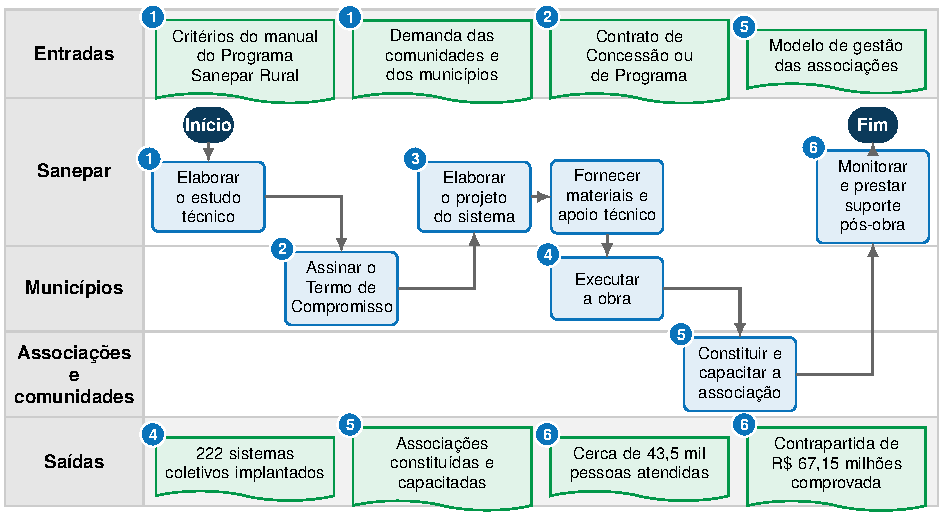
\includegraphics[width=15.96cm]{figuras/g-raias-3224.pdf}
  \fonteMOP{Fonte: IAT (2026), com base em IAT (2026b) e SANEPAR ([s.d.]).}
  % Texto alternativo: Fluxograma em raias da Sanepar, dos municípios e das associações, do estudo técnico ao suporte pós-obra, com as entradas no topo e as saídas na base.
\end{figure}

\phantomsection
\subsubsection*{4.1 Etapa 1: Levantamento técnico e estudo de engenharia}

\textbf{Atividades:} levantamento das condições da comunidade e estudo técnico de engenharia do sistema.

\textbf{Entradas:} demanda da comunidade e do município; critérios do manual do programa.

\textbf{Responsáveis:} Sanepar (executa e aprova); município (consultado).

\textbf{Produto:} estudo técnico da comunidade.

\phantomsection
\subsubsection*{4.2 Etapa 2: Termo de Compromisso com o município}

\textbf{Atividades:} formalização da parceria por Termo de Compromisso e Responsabilidade vinculado ao Contrato de Concessão ou de Programa, com as obrigações de cada parte.

\textbf{Entradas:} estudo técnico; Contrato de Concessão ou de Programa vigente.

\textbf{Responsáveis:} Sanepar e município (executam); Sanepar (aprova).

\textbf{Produto:} Termo de Compromisso e Responsabilidade assinado.

\phantomsection
\subsubsection*{4.3 Etapa 3: Projetos de engenharia}

\textbf{Atividades:} elaboração do projeto de engenharia do sistema de abastecimento de água.

\textbf{Entradas:} estudo técnico; Termo de Compromisso.

\textbf{Responsáveis:} Sanepar (executa e aprova); município (informado).

\textbf{Produto:} projeto do sistema.

\phantomsection
\subsubsection*{4.4 Etapa 4: Execução das obras com apoio da Sanepar}

\textbf{Atividades:} fornecimento dos materiais hidráulicos pela Sanepar; execução das obras pelo município, diretamente ou por contratação própria, com apoio técnico da companhia.

\textbf{Entradas:} projeto aprovado; materiais; outorga e licenças, quando exigidas.

\textbf{Responsáveis:} município (executa a obra); Sanepar (fornece os materiais, presta apoio técnico e aprova a obra).

\textbf{Produto:} sistema implantado.

\phantomsection
\subsubsection*{4.5 Etapa 5: Organização comunitária e capacitação}

\textbf{Atividades:} apoio à constituição da associação de moradores; capacitação em uso racional da água, higiene e manutenção preventiva; educação ambiental.

\textbf{Entradas:} comunidade mobilizada; modelo de gestão.

\textbf{Responsáveis:} Sanepar (executa e aprova); comunidade (executa); IAT (consultado quanto ao modelo de gestão).

\textbf{Produto:} associação constituída e capacitada.

\phantomsection
\subsubsection*{4.6 Etapa 6: Monitoramento e suporte pós-obra}

\textbf{Atividades:} monitoramento pós-obra da qualidade da água e suporte operacional às associações; relatório técnico de cada sistema; reporte anual à UGP dos sistemas implantados, das pessoas atendidas e dos valores aplicados.

\textbf{Entradas:} sistema implantado; associação constituída.

\textbf{Responsáveis:} Sanepar (executa e aprova o relatório técnico); UGP (informada).

\textbf{Produto:} relatório técnico aprovado.

\phantomsection
\subsubsection*{4.7 Modalidade de execução}

O item de custo é o de sistemas coletivos de abastecimento de água com recursos de contrapartida: 222 sistemas ao custo médio de R\$~302.464,42, no total de R\$~67,15 milhões, integralmente com recursos próprios da Sanepar. A execução ocorre por convênio, formalizado em Termo de Compromisso e Responsabilidade entre a Sanepar e cada município, conforme o manual do programa.

As aquisições da Sanepar observam o Regulamento de Licitações e Contratos da companhia, e as obras contratadas pelos municípios, a legislação de licitações aplicável. A Sanepar comprova à UGP os valores aplicados e os sistemas implantados, para registro da contrapartida.

\pendencia{Confirmar com a UGP e o Banco Mundial se as aquisições e as obras financiadas com contrapartida seguem as regras da Sanepar e dos municípios e quais requisitos do Programa se aplicam.}

\phantomsection
\addcontentsline{toc}{subsection}{5. Matriz de responsabilidades}
\subsection*{5. Matriz de responsabilidades}

O Quadro~\ref{raci-3224} apresenta o papel de cada parte em cada etapa.

\begin{quadro}[H]
  \caption{Matriz de responsabilidades do Programa Sanepar Rural}\label{raci-3224}
  \footnotesize\renewcommand{\arraystretch}{1.25}\setlength{\tabcolsep}{3pt}
  \begin{tabular}{>{\raggedright\arraybackslash}p{\dimexpr 0.2536\linewidth-2\tabcolsep\relax}>{\centering\arraybackslash}p{\dimexpr 0.0882\linewidth-2\tabcolsep\relax}>{\centering\arraybackslash}p{\dimexpr 0.0882\linewidth-2\tabcolsep\relax}>{\centering\arraybackslash}p{\dimexpr 0.0882\linewidth-2\tabcolsep\relax}>{\centering\arraybackslash}p{\dimexpr 0.0882\linewidth-2\tabcolsep\relax}>{\centering\arraybackslash}p{\dimexpr 0.0882\linewidth-2\tabcolsep\relax}>{\centering\arraybackslash}p{\dimexpr 0.0882\linewidth-2\tabcolsep\relax}>{\centering\arraybackslash}p{\dimexpr 0.2173\linewidth-2\tabcolsep\relax}}
    \rowcolor{azulEscuro}\textcolor{white}{\textbf{Parte}} & \textcolor{white}{\textbf{E1}} & \textcolor{white}{\textbf{E2}} & \textcolor{white}{\textbf{E3}} & \textcolor{white}{\textbf{E4}} & \textcolor{white}{\textbf{E5}} & \textcolor{white}{\textbf{E6}} & \textcolor{white}{\textbf{Produto final}} \\
    Sanepar & \raci{R} \raci{A} & \raci{R} \raci{A} & \raci{R} \raci{A} & \raci{A} & \raci{R} \raci{A} & \raci{R} \raci{A} & \raci{R} \raci{A} \\ \arrayrulecolor{cinza20}\hline
    \rowcolor{cinza5}Municípios & \raci{C} & \raci{R} & \raci{I} & \raci{R} & \raci{C} & \raci{I} & \raci{I} \\ \arrayrulecolor{cinza20}\hline
    Comunidades e associações & \raci{C} & – & – & \raci{I} & \raci{R} & \raci{C} & \raci{R} \\ \arrayrulecolor{cinza20}\hline
    \rowcolor{cinza5}IAT & – & – & – & – & \raci{C} & \raci{I} & \raci{I} \\ \arrayrulecolor{cinza20}\hline
    UGP & – & – & – & – & – & \raci{I} & \raci{I} \\ \noalign{\global\arrayrulewidth=1pt}\arrayrulecolor{azulEscuro}\hline\noalign{\global\arrayrulewidth=0.4pt}
  \end{tabular}
  \fonteMOP{Fonte: IAT (2026).}
  \notaMOP{Nota: E1 a E6 correspondem às Etapas 1 a 6 do item 4. \raci{R} executa (pode haver mais de um); \raci{A} aprova ou valida o produto (um por etapa); \raci{C} é consultado previamente; \raci{I} é informado posteriormente. Produto final: sistemas implantados e pessoas atendidas.}
\end{quadro}

\phantomsection
\addcontentsline{toc}{subsection}{6. Metas, indicadores e comprovação}
\subsection*{6. Metas, indicadores e comprovação}

A meta é a implantação de 222 sistemas de 2027 a 2031 (Quadro~\ref{metas-3224}).

\begin{quadro}[H]
  \caption{Metas anuais do Programa Sanepar Rural}\label{metas-3224}
  \footnotesize\renewcommand{\arraystretch}{1.25}\setlength{\tabcolsep}{3pt}
  \begin{tabular}{>{\raggedright\arraybackslash}p{\dimexpr 0.2095\linewidth-2\tabcolsep\relax}>{\raggedright\arraybackslash}p{\dimexpr 0.1268\linewidth-2\tabcolsep\relax}>{\raggedleft\arraybackslash}p{\dimexpr 0.0794\linewidth-2\tabcolsep\relax}>{\raggedleft\arraybackslash}p{\dimexpr 0.0794\linewidth-2\tabcolsep\relax}>{\raggedleft\arraybackslash}p{\dimexpr 0.0794\linewidth-2\tabcolsep\relax}>{\raggedleft\arraybackslash}p{\dimexpr 0.0794\linewidth-2\tabcolsep\relax}>{\raggedleft\arraybackslash}p{\dimexpr 0.0794\linewidth-2\tabcolsep\relax}>{\raggedleft\arraybackslash}p{\dimexpr 0.0794\linewidth-2\tabcolsep\relax}>{\raggedleft\arraybackslash}p{\dimexpr 0.0794\linewidth-2\tabcolsep\relax}>{\raggedleft\arraybackslash}p{\dimexpr 0.1081\linewidth-2\tabcolsep\relax}}
    \rowcolor{azulEscuro}\textcolor{white}{\textbf{Produto}} & \textcolor{white}{\textbf{Unidade}} & \centering\arraybackslash \textcolor{white}{\textbf{Ano 1}} & \centering\arraybackslash \textcolor{white}{\textbf{Ano 2}} & \centering\arraybackslash \textcolor{white}{\textbf{Ano 3}} & \centering\arraybackslash \textcolor{white}{\textbf{Ano 4}} & \centering\arraybackslash \textcolor{white}{\textbf{Ano 5}} & \centering\arraybackslash \textcolor{white}{\textbf{Ano 6}} & \centering\arraybackslash \textcolor{white}{\textbf{Ano 7}} & \centering\arraybackslash \textcolor{white}{\textbf{Total}} \\
    Sistemas coletivos de abastecimento de água & sistemas & 45 & 41 & 42 & 43 & 51 & – & – & 222 \\ \arrayrulecolor{cinza20}\hline
    \rowcolor{cinza5}Pessoas atendidas & pessoas & 8.820 & 8.036 & 8.232 & 8.428 & 9.996 & – & – & 43.512 \\ \noalign{\global\arrayrulewidth=1pt}\arrayrulecolor{azulEscuro}\hline\noalign{\global\arrayrulewidth=0.4pt}
  \end{tabular}
  \fonteMOP{Fonte: Planilha PSH\_CUSTO\_Consolidada, versão v2408 (PARANÁ, 2026).}
  \notaMOP{Nota: Ano 1 = 2027 e Ano 7 = 2033. Pessoas estimadas com 70 domicílios por sistema e 2,8 pessoas por domicílio, conforme o indicador do componente.}
\end{quadro}

Os indicadores constam do Quadro~\ref{ind-3224}. A Sanepar informa anualmente à UGP os sistemas implantados, as pessoas atendidas, com desagregação por sexo e para jovens de 15 a 24 anos, e os valores de contrapartida aplicados.

\begin{quadro}[H]
  \caption{Indicadores do Programa Sanepar Rural}\label{ind-3224}
  \footnotesize\renewcommand{\arraystretch}{1.25}\setlength{\tabcolsep}{3pt}
  \begin{tabular}{>{\raggedright\arraybackslash}p{\dimexpr 0.3165\linewidth-2\tabcolsep\relax}>{\raggedright\arraybackslash}p{\dimexpr 0.1378\linewidth-2\tabcolsep\relax}>{\raggedleft\arraybackslash}p{\dimexpr 0.1102\linewidth-2\tabcolsep\relax}>{\raggedleft\arraybackslash}p{\dimexpr 0.1599\linewidth-2\tabcolsep\relax}>{\raggedright\arraybackslash}p{\dimexpr 0.2756\linewidth-2\tabcolsep\relax}}
    \rowcolor{azulEscuro}\textcolor{white}{\textbf{Indicador}} & \textcolor{white}{\textbf{Unidade}} & \centering\arraybackslash \textcolor{white}{\textbf{Linha de base (2025)}} & \centering\arraybackslash \textcolor{white}{\textbf{Meta}} & \textcolor{white}{\textbf{Frequência e fonte dos dados}} \\
    Sistemas implantados pelo Programa Sanepar Rural & sistemas & 0 & 222 & Anual; Sanepar \\ \arrayrulecolor{cinza20}\hline
    \rowcolor{cinza5}Pessoas atendidas com água gerida de forma segura (parcela do indicador do componente) & pessoas & 0 & 43.500 & Anual; Sanepar, com desagregação por sexo e jovens \\ \arrayrulecolor{cinza20}\hline
    Contrapartida aplicada & R\$~milhões & 0 & 67,15 & Anual; Sanepar e UGP \\ \noalign{\global\arrayrulewidth=1pt}\arrayrulecolor{azulEscuro}\hline\noalign{\global\arrayrulewidth=0.4pt}
  \end{tabular}
  \fonteMOP{Fonte: IAT (2026).}
\end{quadro}

\pendencia{O MOP de março atribuía ao Programa Sanepar Rural a meta total do indicador (59.780 pessoas), que inclui os sistemas do IAT. A parcela da Sanepar é de cerca de 43.500 pessoas. Confirmar com a Sanepar e citar o manual do programa com título, versão e data.}

Os critérios de aceite e as evidências de cada produto constam do Quadro~\ref{aceite-3224}. A evidência de conclusão de cada sistema é o relatório técnico aprovado pela Sanepar.

\begin{quadro}[H]
  \caption{Critérios de aceite e evidências do Programa Sanepar Rural}\label{aceite-3224}
  \footnotesize\renewcommand{\arraystretch}{1.25}\setlength{\tabcolsep}{5pt}
  \begin{tabular}{>{\raggedright\arraybackslash}p{\dimexpr 0.2150\linewidth-2\tabcolsep\relax}>{\raggedright\arraybackslash}p{\dimexpr 0.3386\linewidth-2\tabcolsep\relax}>{\raggedright\arraybackslash}p{\dimexpr 0.2921\linewidth-2\tabcolsep\relax}>{\raggedright\arraybackslash}p{\dimexpr 0.1543\linewidth-2\tabcolsep\relax}}
    \rowcolor{azulEscuro}\textcolor{white}{\textbf{Produto}} & \textcolor{white}{\textbf{Critério de aceite}} & \textcolor{white}{\textbf{Evidência de comprovação}} & \textcolor{white}{\textbf{Responsável pela validação}} \\
    Termo de Compromisso & Assinado pela Sanepar e pelo município & Termo assinado & Sanepar \\ \arrayrulecolor{cinza20}\hline
    \rowcolor{cinza5}Projeto do sistema & Aprovado conforme as normas da Sanepar & Projeto aprovado & Sanepar \\ \arrayrulecolor{cinza20}\hline
    Sistema implantado & Obra concluída e em operação, com água conforme o padrão de potabilidade & Relatório técnico aprovado; laudos de qualidade da água & Sanepar \\ \arrayrulecolor{cinza20}\hline
    \rowcolor{cinza5}Associação capacitada & Associação constituída e capacitada em operação e manutenção & Registro da associação; listas de presença & Sanepar \\ \arrayrulecolor{cinza20}\hline
    Contrapartida comprovada & Valores aplicados registrados por sistema & Relatório financeiro da Sanepar & UGP \\ \noalign{\global\arrayrulewidth=1pt}\arrayrulecolor{azulEscuro}\hline\noalign{\global\arrayrulewidth=0.4pt}
  \end{tabular}
  \fonteMOP{Fonte: IAT (2026).}
\end{quadro}

\phantomsection
\addcontentsline{toc}{subsection}{7. Gestão de riscos e impactos ambientais e sociais}
\subsection*{7. Gestão de riscos e impactos ambientais e sociais}

Os riscos são análogos aos dos sistemas implantados pelo IAT: impactos temporários das obras, segurança dos trabalhadores e da comunidade, uso das áreas das estruturas, qualidade da água e participação das comunidades. Por integrar o Programa, a ação observa os instrumentos do Caderno AS (Quadro~\ref{nas-3224}).

\begin{quadro}[H]
  \caption{Aplicação das Normas Ambientais e Sociais ao Programa Sanepar Rural}\label{nas-3224}
  \footnotesize\renewcommand{\arraystretch}{1.25}\setlength{\tabcolsep}{5pt}
  \begin{tabular}{>{\raggedright\arraybackslash}p{\dimexpr 0.1874\linewidth-2\tabcolsep\relax}>{\raggedright\arraybackslash}p{\dimexpr 0.3716\linewidth-2\tabcolsep\relax}>{\raggedright\arraybackslash}p{\dimexpr 0.4410\linewidth-2\tabcolsep\relax}}
    \rowcolor{azulEscuro}\textcolor{white}{\textbf{NAS}} & \textcolor{white}{\textbf{Aplicação à ação}} & \textcolor{white}{\textbf{Medidas e instrumentos}} \\
    NAS 1 – Avaliação e gestão de riscos & Obras em cada comunidade & Triagem socioambiental; licenças, quando exigidas; procedimentos ambientais da Sanepar \\ \arrayrulecolor{cinza20}\hline
    \rowcolor{cinza5}NAS 2 – Condições de trabalho & Trabalhadores das obras municipais e da Sanepar & Uso de EPI e protocolos de saúde e segurança do trabalho \\ \arrayrulecolor{cinza20}\hline
    NAS 3 – Eficiência de recursos e prevenção da poluição & Captação de água e resíduos de obra & Outorga; controle de perdas; destinação adequada dos resíduos \\ \arrayrulecolor{cinza20}\hline
    \rowcolor{cinza5}NAS 4 – Saúde e segurança da comunidade & Valas, trânsito de máquinas e qualidade da água & Sinalização das obras; monitoramento da qualidade da água pela Sanepar \\ \arrayrulecolor{cinza20}\hline
    NAS 5 – Aquisição de terras & Áreas para captação e reservação & Verificação da titularidade e anuência; ausência de reassentamento involuntário \\ \arrayrulecolor{cinza20}\hline
    \rowcolor{cinza5}NAS 10 – Engajamento das partes interessadas & Comunidades e associações & Mobilização e organização comunitária; canal de atendimento da Sanepar e Mecanismo de Queixas e Reclamações do Programa \\ \noalign{\global\arrayrulewidth=1pt}\arrayrulecolor{azulEscuro}\hline\noalign{\global\arrayrulewidth=0.4pt}
  \end{tabular}
  \fonteMOP{Fonte: IAT (2026), com base nos instrumentos do Caderno AS.}
  \notaMOP{Nota: as NAS 6, 7 e 8 são verificadas na triagem de cada sistema.}
\end{quadro}

\pendencia{Confirmar com a UGP quais instrumentos do Caderno AS se aplicam às ações executadas com recursos de contrapartida.}

\phantomsection
\addcontentsline{toc}{subsection}{8. Cronograma}
\subsection*{8. Cronograma}

A ação ocorre de 2027 a 2031 (Figura~\ref{crono-3224}): 45 sistemas em 2027, 41 em 2028, 42 em 2029, 43 em 2030 e 51 em 2031. Os estudos, os termos e os projetos de cada ano antecedem as obras do ano seguinte, e o suporte pós-obra prossegue como atividade de rotina da Sanepar após 2031.

\begin{figure}[H]
  \centering
  \caption{Cronograma das etapas e das entregas do Programa Sanepar Rural}\label{crono-3224}
  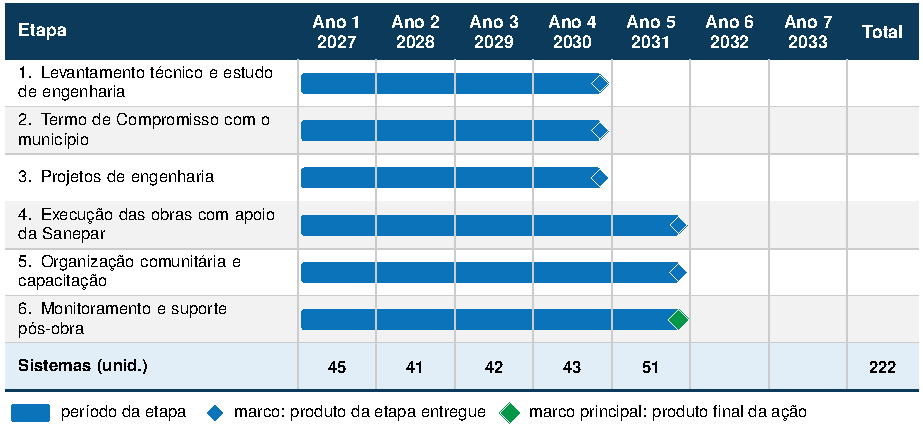
\includegraphics[width=15.64cm]{figuras/g-crono-3224.pdf}
  \fonteMOP{Fonte: IAT (2026), com quantidades da planilha PSH\_CUSTO\_Consolidada (PARANÁ, 2026).}
  % Texto alternativo: Cronograma anual de 2027 a 2033 com as etapas e as quantidades a entregar do Programa Sanepar Rural.
\end{figure}

\phantomsection
\addcontentsline{toc}{subsection}{9. Interfaces e dependências}
\subsection*{9. Interfaces e dependências}

A ação recebe dos modelos de gestão o arranjo aplicável às associações de moradores e da política estadual de saneamento rural as diretrizes setoriais. Fornece à UGP o número de pessoas atendidas e a comprovação da contrapartida e alimenta o indicador de pessoas atendidas com água gerida de forma segura (Figura~\ref{interf-3224}).

\begin{figure}[H]
  \centering
  \caption{Interfaces e dependências do Programa Sanepar Rural}\label{interf-3224}
  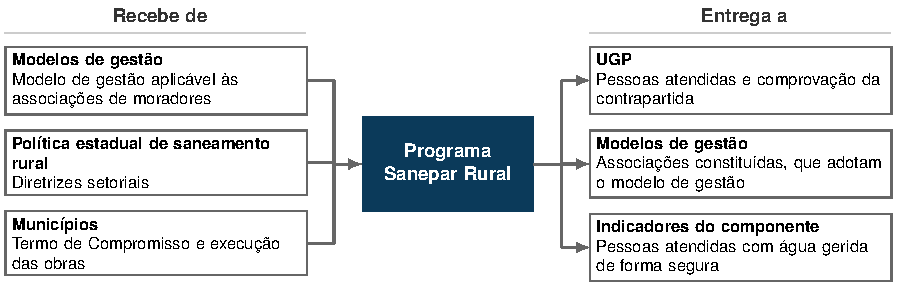
\includegraphics[width=15.30cm]{figuras/g-interf-3224.pdf}
  \fonteMOP{Fonte: IAT (2026).}
  % Texto alternativo: Diagrama das interfaces do Programa Sanepar Rural: insumos recebidos de outras partes do Programa e produtos entregues a elas.
\end{figure}

\phantomsection
\addcontentsline{toc}{subsection}{10. Documentos complementares}
\subsection*{10. Documentos complementares}

\begin{itemize}
  \item Manual do Programa Sanepar Rural (SANEPAR, [s.d.]);
  \item Contratos de Concessão e de Programa entre a Sanepar e os municípios;
  \item Modelo do Termo de Compromisso e Responsabilidade;
  \item Regulamento de Licitações e Contratos da Sanepar;
  \item Portaria GM/MS nº~888/2021 (padrão de potabilidade);
  \item Caderno AS.
\end{itemize}
